\documentclass[A4paper,12pt]{report}
\usepackage[centertags]{amsmath}
\usepackage{chapterbib}
\usepackage{amsfonts}
\usepackage{amssymb}
\usepackage{amsthm}
\usepackage{lmodern}
\usepackage{epsfig}
\usepackage[table,xcdraw]{xcolor}
\usepackage{graphicx}
\usepackage{newlfont}
\usepackage{tabularx}
\usepackage{pdflscape}
\usepackage{hyperref}
\usepackage{mathtools}
\usepackage{amsmath}
\usepackage{graphicx}
\usepackage{sectsty}
\usepackage{amsmath,latexsym}
\usepackage{amssymb}
\usepackage{setspace}
\usepackage{amsfonts}
\usepackage{amsthm}
\usepackage{float}
\usepackage{tikz}
\usepackage{epsfig}
\usepackage{epstopdf}
\usepackage{textpos}
\usepackage{placeins}
\usepackage{caption}
\usepackage{subcaption}
\usepackage{color}
\usepackage{tocloft}
\usepackage{setspace,kantlipsum}
\usepackage[hmargin=1.4in,hmargin=1.4in]{geometry}
\usepackage{mathptmx}
\usepackage{titlesec}
\usepackage{lscape}
\usepackage{booktabs,threeparttable}
\usepackage{algorithm}
\usepackage{algpseudocode}
\usepackage{multirow}

\newgeometry{left=1.5in,right=1.0in,top=1in,bottom=1in}
% THEOREMS ---------------------------------------------------------------
\theoremstyle{plain}
\newtheorem{thm}{Theorem}[section]
\newtheorem{cor}[thm]{Corollary}
\newtheorem{lem}[thm]{Lemma}
\newtheorem{Proposition}[thm]{Proposition}
\newtheorem{opn}[thm]{}
\renewcommand\cftchapfont{\fontsize{13}{13}\selectfont\bfseries}
\renewcommand\cftsecfont{\fontsize{13}{13}\selectfont}
\renewcommand\cftsubsecfont{\fontsize{13}{13}\selectfont}
\titleformat{\chapter}[display]{\filcenter\bfseries\fontsize{20}{20}\selectfont}{{\chaptername} \thechapter}{0pt}{\vskip 0pt}
\titlespacing*{\chapter}{0cm}{-\topskip}{10pt}[0pt]
\theoremstyle{definition}
\newtheorem{defn}{Definition}[section]
\renewcommand\listfigurename{\hfill \LARGE{List of Figures} \hfill}
\renewcommand\listtablename{\hfill \LARGE{List of Tables} \hfill}
\theoremstyle{remark}
\newtheorem{rem}{Remark}[section]
\renewcommand{\cftpartleader}{\cftdotfill{\cftdotsep}}
\renewcommand{\cftchapleader}{\cftdotfill{\cftdotsep}}
\renewcommand\bibname{References}
\renewcommand\cftbeforetoctitleskip{0cm}
\renewcommand\cftbeforeloftitleskip{0cm}
\renewcommand\cftbeforelottitleskip{0cm}
\numberwithin{equation}{section}
\renewcommand{\theequation}{\thesection.\arabic{equation}}
\renewcommand{\contentsname}{\hfill \LARGE{Table of Contents}\hfill}
\titleformat*{\section}{\large\bfseries}
\titleformat*{\subsection}{\fontsize{4.5mm}{4.5mm}\selectfont}
\renewcommand*\cftfigpresnum{Figure}
\settowidth{\cftfignumwidth}{\cftfigpresnum}
\renewcommand{\cftfigaftersnumb}{\quad\quad~}
\newlength\mylen
\settowidth{\mylen}{\cfttabpresnum\cfttabaftersnum}
\addtolength{\cfttabnumwidth}{\mylen}
\setlength\cfttabindent{0pt}
\setlength\cftfigindent{0pt}
\newcolumntype{a}{>{\columncolor{classicrose}}S{p{8.5cm}}}
\addtocontents{toc}{\protect{\pdfbookmark[0]{\contentsname}{toc}}}
\addtocontents{lof}{\protect{\pdfbookmark[0]{\listfigurename}{lof}}}
\addtocontents{lot}{\protect{\pdfbookmark[0]{\listtablename}{lot}}}

\begin{document}
\pagenumbering{roman}
\thispagestyle{empty}
\pdfbookmark[0]{\@Title Page}{Title Page}
\begin{center}
{\Huge{Risk-Aware Service Function Chain Placement Using Maskable Proximal Policy Optimization with Graph Neural Networks}}
\end{center}
\vspace{0.1in}
\begin{center}
%\includegraphics[width=4.6cm, height=4.6cm]{comsats.eps}\\
\vspace{.8in}
\Large{MS Thesis}\\
\large{ by}\\
\Large {Ali Raheel}\\
\vspace{0.35in}
CIIT/SP22-MSCS-001/ISB\\
\vspace{2in}
\Large {\textbf{COMSATS University Islamabad\\
Pakistan}}\\
\vspace{0.2in}
\Large{\textbf{Spring 2025}}
\end{center}

\newpage
\vspace{-1in}
\begin{center}
%\raisebox{-3\baselineskip}{\includegraphics[width=4.6cm, height=4.6cm]{comsats.eps}}
\end{center}

\begin{center}
\vspace{0.1in}
\LARGE{Risk-Aware Service Function Chain Placement Using Maskable Proximal Policy Optimization with Graph Neural Networks} \\
\vspace{0.5in}
\Large{A thesis submitted to}\\
\vspace{0in}
\Large{COMSATS University Islamabad}\\
\vspace{0.3in}
\large{In partial fulfillment\\
of the requirement for the degree of}\\
\vspace{0.3in}
\large{Master of Science}\\
\large{in}\\
\large{Computer Science}\\
\vspace{0.2in}
\normalsize{by}\\
\large{Ali Raheel\\
\vspace{0.1in}
CIIT/SP22-MSCS-001/ISB}\\
\vspace{0.2in}
\large{Department of Computer Science}\\
\large{Faculty of Information Technology}\\
\vspace{0.3in}
\Large {\textbf{COMSATS University Islamabad\\
Pakistan}}\\
\vspace{0.2in}
\Large{\textbf{Spring 2025}}
\end{center}


\newpage
\begin{center}
\LARGE{Risk-Aware Service Function Chain Placement Using Maskable Proximal Policy Optimization with Graph Neural Networks}\\
\end{center}
\vspace{0.2in}
\noindent\large{This thesis is submitted to the Department of Computer Science in partial fulfillment of the requirement for the award of degree of Master of Science in Computer Science}
\vspace{0.02in}
\begin{table}[!ht]
\centering
{\setlength{\arrayrulewidth}{.5mm}
\setlength{\tabcolsep}{53pt}
\renewcommand{\arraystretch}{2}
\begin{tabular}{|c|c|}
\hline
\rowcolor[HTML]{656565}
 \large{Name} &\large{Registration Number}  \\
 \hline
Ali Raheel & CIIT/SP22-MSCS-001/ISB \\ \hline
\end{tabular}
}
\vspace{0.3in}
\end{table}
\vspace{2in}

\noindent\large{\textbf{Supervisor}}
\begin{flushleft}
\vspace{0.3in}
\large{Dr. Supervisor Name\\
\vspace{0.1in}
Associate Professor,\\
Department of Computer Science\\
\vspace{0.1in}
COMSATS University Islamabad\\

\vspace{0.2in}
May, 2025 }
\end{flushleft}
\newpage
\begin{spacing}{1.5}
\begin{center}
\LARGE{\textbf{{Certificate of Approval}}}\\
\end{center}

\begin{center}
\normalsize {This thesis titled}\\
\LARGE{Risk-Aware Service Function Chain Placement Using Maskable Proximal Policy Optimization with Graph Neural Networks}\\
\normalsize {By\\
Ali Raheel\\

CIIT/SP22-MSCS-001/ISB\\

Has been approved}\\

\end{center}

\begin{center}
\normalsize {For COMSATS University Islamabad.}\\
\end{center}

\vspace{0.1in}
\noindent \normalsize {External Examiner:}\line(1,0){260}
\begin{center}
\normalsize {Dr. External Examiner}\\
University Name\\
\end{center}
\vspace{0.1in}
\normalsize {Supervisor:}\line(1,0){310}
\begin{center}
\normalsize {Dr. Supervisor Name\\
Department of Computer Science, COMSATS University Islamabad}
\end{center}
\vspace{0.1in}
\normalsize {Head of Department:}\line(1,0){260}
\begin{center}
\normalsize {Prof. Dr. Head of Department\\
Department of Computer Science, COMSATS University Islamabad}
\end{center}

\newpage
\begin{center}
\LARGE{\textbf{Author's Declaration}}\\
\vspace{0.1in}
\end{center}
\noindent\normalsize{I, Ali Raheel, Registration No. CIIT/SP22-MSCS-001/ISB, hereby declare that I have produced the work presented in this thesis during the scheduled period of study. I also declare that I have not taken any material from any source except as referred to wherever due, and that the amount of plagiarism is within an acceptable range. If a violation of HEC rules on research has occurred in this thesis, I shall be liable to punishable action under the plagiarism rules of HEC.}\\

\vspace{1in}


Date:\line(1,0){80}\hfill\line(1,0){150}
\begin{flushright}
Ali Raheel\\
CIIT/SP22-MSCS-001/ISB
\end{flushright}

\newpage

\begin{center}
\LARGE{\textbf{Certificate}}\\
\vspace{0.2in}
\end{center}
It is certified that Ali Raheel, CIIT/SP22-MSCS-001/ISB, has carried out all the work related to this thesis under my supervision at the Department of Computer Science, COMSATS University Islamabad, and the work fulfills the requirement for the award of the MS degree.\\


\vspace{1in}
Date:\line(1,0){80}\\

\vspace{0.5in}
\begin{flushright}
\begin{tabular}{@{}l@{}}
Supervisor\\
\vspace{0.3in}
\\
\line(1,0){80}\\
Dr. Supervisor Name\\
Associate Professor,\\
Computer Science,\\
COMSATS University Islamabad
\end{tabular}
\end{flushright}


\newpage
\begin{center}
\textbf{\LARGE{Dedication}}\\

\vspace{.5in}

\Large{To My Parents, Family, and All Who Seek Knowledge}


\end{center}


\newpage
\begin{center}
\LARGE\textbf{{Acknowledgements}}\\
\end{center}
\vspace{0.3in}
\begin{center}
\textbf{Praise be to ALLAH, the Cherisher and Lord\\of the World, Most Gracious and Most Merciful}
\end{center}
\normalsize{First and foremost, I would like to thank ALLAH Almighty (the Most Beneficent and Most Merciful) for granting me the strength, knowledge, ability, and opportunity to undertake this research and to persevere and complete it satisfactorily. Without His countless blessings, this achievement would not have been possible. May His peace and blessings be upon His messenger Hazrat Muhammad (PBUH), upon his family, companions, and all who follow him.

I wish to express my deepest and most sincere gratitude to my supervisor, Dr. Supervisor Name, for his invaluable guidance, continuous encouragement, and insightful feedback throughout the course of this research. His expertise in computer networks and machine learning has been instrumental in shaping this work. I am deeply indebted to him for the time and effort he invested in my academic and professional development.

I would also like to acknowledge the Department of Computer Science at COMSATS University Islamabad for providing an excellent academic environment and computational resources that made this research possible.

My heartfelt gratitude goes to my parents, whose unconditional love, prayers, and sacrifices have been a constant source of motivation. Their unwavering belief in me has been my greatest strength throughout this journey.

I am also thankful to my colleagues and friends who provided moral support, constructive discussions, and encouragement throughout my studies.

Finally, I acknowledge the open-source communities behind Stable-Baselines3, PyTorch Geometric, Gymnasium, and NetworkX, whose tools formed the backbone of the software infrastructure of this research.}

\vspace{0.5in}
\hspace{265pt}Ali Raheel

\hspace{240pt}CIIT/SP22-MSCS-001/ISB


\newpage
\begin{center}
\LARGE{\textbf{\textbf{Abstract}}}
\end{center}
\begin{center}
\Large{Risk-Aware Service Function Chain Placement Using Maskable Proximal Policy Optimization with Graph Neural Networks}\\
\Large{By}\\
\Large{Ali Raheel}
\end{center}

The rapid proliferation of Network Function Virtualization (NFV) and Software-Defined Networking (SDN) has transformed the way network services are deployed and managed. Service Function Chains (SFCs) — ordered sequences of Virtual Network Functions (VNFs) — must be efficiently embedded onto substrate networks while satisfying stringent resource, latency, bandwidth, and security constraints. Classical placement algorithms are computationally expensive or rely on hand-crafted heuristics that fail to generalize across diverse network conditions. Furthermore, existing methods rarely account for the operational risk introduced by co-locating VNFs, security vulnerabilities, and stochastic failure events.

This thesis proposes a risk-aware deep reinforcement learning framework for SFC placement that addresses these shortcomings. The framework models the placement problem as a Markov Decision Process (MDP) and trains a Maskable Proximal Policy Optimization (Maskable PPO) agent to sequentially place VNFs onto substrate nodes. Action masking is employed to strictly enforce all feasibility constraints — including resource availability, latency budget reservation, bandwidth along shortest paths, security requirements, and hard isolation — preventing the agent from exploring infeasible placements entirely.

A key contribution of this work is a topology-aware policy that incorporates a Graph Neural Network (GNN) feature extractor. Three GNN architectures are investigated: Graph Convolutional Networks (GCN), Graph Attention Networks (GAT), and GraphSAGE. The GNN processes real-time substrate node embeddings through multiple message-passing layers, followed by an attention-weighted graph-level aggregation, and fuses the result with a global context vector encoding the current SFC request properties. This design enables the agent to learn topology-dependent placement strategies without requiring the network size to be fixed at training time.

A novel composite risk model is introduced that quantifies operational risk as a weighted combination of VNF tenancy, SFC tenancy, inverse node security, a stochastic incident process, and time-exposure. The incident component models security breaches and failure events as Bernoulli trials whose probability depends on node load, security posture, and incident pressure accumulated from past events. The risk integral is coupled to the reward signal via a tunable penalty coefficient, steering the agent toward placements that are both efficient and operationally resilient.

Experimental evaluation on a 25-node substrate network with 1000 SFC requests demonstrates that the Maskable PPO agent achieves competitive acceptance ratios relative to a risk-minimizing Best-Fit heuristic baseline, while incurring lower average risk integrals and fewer realized security incidents. The windowed acceptance ratio reward modifier further stabilizes training by providing curriculum-style feedback that adapts the reward magnitude to recent performance. Comprehensive metrics including acceptance ratio, average end-to-end latency, substrate utilization, SFC/VNF tenancy, and realized incident rates are reported and analyzed.

\newpage
\tableofcontents
\clearpage
\listoffigures
\clearpage
{\let\oldnumberline\numberline%
\renewcommand{\numberline}{\tablename~\oldnumberline}%
\listoftables}
\clearpage


\pagenumbering{arabic}
% ===========================================================================
\chapter{Introduction}
% ===========================================================================

\section{Background}

The last decade has witnessed a profound transformation in the architecture of communication networks, driven by two paradigm-shifting technologies: Software-Defined Networking (SDN) and Network Function Virtualization (NFV). Traditional networks relied on dedicated, proprietary hardware appliances to implement network functions such as firewalls, load balancers, intrusion detection systems, and deep packet inspection engines. These ``middleboxes'' were expensive to procure, rigid in their placement, and difficult to manage at scale \cite{mijumbi2016}.

SDN decouples the control plane from the data plane, centralizing network intelligence in a logically centralized controller that programs forwarding rules across the network infrastructure via standardized protocols such as OpenFlow \cite{mckeown2008}. This separation introduces unprecedented programmability and flexibility in network management.

NFV complements SDN by decoupling network functions from the dedicated hardware on which they were traditionally implemented, running them instead as software instances — Virtual Network Functions (VNFs) — on commodity servers in data centers \cite{etsi2013}. NFV allows network operators to instantiate, scale, migrate, and terminate VNFs dynamically in response to traffic demands, dramatically reducing both capital expenditure (CapEx) and operational expenditure (OpEx).

The convergence of SDN and NFV has given rise to the concept of \textit{Service Function Chaining} (SFC), wherein ordered sequences of VNFs are composed to implement end-to-end network services \cite{halpern2015}. For example, a corporate network might route traffic through a firewall, then a WAN optimizer, then a load balancer before it reaches its destination. The ability to specify, instantiate, and route traffic through such chains programmatically is a cornerstone of modern cloud-native and 5G network architectures \cite{nfv5g2017}.

\section{The SFC Placement Problem}

Given the flexibility offered by NFV/SDN, a fundamental challenge emerges: \textit{where} should the VNFs that comprise an SFC be deployed on the physical substrate network? This \textbf{SFC Placement Problem} (also called the VNF Embedding Problem or NFV Resource Allocation Problem) requires simultaneously satisfying a complex set of constraints:

\begin{itemize}
  \item \textbf{Resource constraints:} Each substrate node has finite CPU, RAM, and storage capacity; the aggregate demands of all VNFs placed on a node must not exceed its available resources.
  \item \textbf{Latency constraints:} The accumulated end-to-end latency along the path from the first to the last VNF must not exceed the SFC's maximum latency requirement.
  \item \textbf{Bandwidth constraints:} Each link along the path between consecutive VNFs must have sufficient residual bandwidth to carry the SFC traffic.
  \item \textbf{Security constraints:} Each substrate node on which a VNF is placed must meet the minimum security score required by the SFC.
  \item \textbf{Isolation constraints:} Some SFCs require \textit{hard isolation}, meaning their VNFs must not share substrate nodes with VNFs of other SFCs.
\end{itemize}

The SFC placement problem has been shown to be NP-hard in general \cite{dolev2013}, as it encompasses variants of the Virtual Network Embedding (VNE) problem, which subsumes bin-packing and graph isomorphism \cite{yu2008}. Consequently, exact algorithms are intractable for large-scale networks, and practical solutions must rely on approximations, heuristics, or learning-based approaches.

\section{Limitations of Existing Approaches}

Classical approaches to SFC placement fall into three broad categories:

\textbf{Exact methods}, such as Integer Linear Programming (ILP) \cite{cohen2015}, guarantee optimal solutions but scale exponentially with problem size, making them suitable only for small networks or offline planning scenarios. Dynamic programming approaches (e.g., Viterbi-style trellis methods) offer polynomial-time optimality for restricted objective functions but still do not scale to large substrate networks with hundreds of nodes under continuously arriving requests.

\textbf{Heuristic methods}, such as First-Fit and Best-Fit algorithms, make locally greedy decisions and run efficiently in practice but lack any global optimization perspective. They typically optimize a single criterion (e.g., resource waste) while ignoring others (e.g., risk, security diversity, future load), and their performance degrades significantly under high load.

\textbf{Meta-heuristic and evolutionary methods} \cite{rankothge2017}, such as genetic algorithms and simulated annealing, offer better solution quality than greedy heuristics but require careful hyperparameter tuning, suffer from slow convergence, and are difficult to adapt online to real-time request arrivals.

A fundamental limitation shared by all of the above is that they \textit{do not learn from experience}. Each incoming SFC request is solved in isolation, without leveraging patterns learned from prior requests. Moreover, virtually no existing practical method incorporates a realistic model of operational risk — the possibility that VNF co-location, node security vulnerabilities, or accumulated load may lead to security incidents, failures, or degraded service quality over time.

\section{Reinforcement Learning for SFC Placement}

Reinforcement Learning (RL) offers a compelling alternative: an agent learns a placement policy through interaction with the environment, receiving reward signals that encode the desired optimization objectives. The agent improves its policy over many episodes, ultimately learning to make globally informed placement decisions that account for long-term consequences \cite{mao2016}.

Recent work has demonstrated the viability of deep RL for network resource management problems, including virtual machine placement \cite{mao2016}, VNE \cite{yan2020}, and SFC embedding \cite{heo2020}. A key advantage of RL-based approaches is their ability to generalize: once trained, the policy executes in milliseconds, making it highly suitable for online, real-time placement. Furthermore, RL policies can naturally encode multi-objective trade-offs through the reward function, incorporating resource efficiency, latency minimization, security, and risk simultaneously.

However, applying standard RL to combinatorial placement problems with hard constraints presents a major challenge: the agent may waste a significant fraction of training exploring infeasible actions, leading to slow convergence and unstable learning. \textbf{Action masking} \cite{vinyals2019, huang2020} is a well-established technique that addresses this by dynamically pruning the action space to include only feasible choices, drastically improving sample efficiency and guaranteeing constraint satisfaction during both training and inference.

\section{Graph Neural Networks for Topology-Aware Placement}

The substrate network is inherently a graph, and the placement decision for each VNF is fundamentally topology-dependent: the latency and bandwidth between nodes, the load distribution across the graph, and the structural position of candidate nodes all influence the quality of a placement. Standard multi-layer perceptrons (MLPs) treat node features in isolation and are unable to capture these relational, graph-structural dependencies.

Graph Neural Networks (GNNs) \cite{kipf2017, velickovic2018, hamilton2017} learn node representations by aggregating information from neighborhood nodes through iterative message passing, naturally encoding the topological context of each node. Embedding a GNN into the policy network of an RL agent endows it with topology awareness, enabling it to reason about placement decisions in the context of the entire network graph \cite{lotfi2022}.

\section{Research Motivation and Objectives}

Despite significant progress in applying RL and GNNs to network resource management, several gaps remain:

\begin{enumerate}
  \item \textbf{Operational risk is largely ignored.} Existing RL-based SFC placement methods optimize for acceptance ratio, latency, and resource utilization, but do not model the security and reliability risk associated with specific placements.
  \item \textbf{Stochastic failure dynamics are not modeled.} Real networks experience security incidents and node failures whose probability depends on load, security posture, and historical incident pressure. Ignoring this leads to placements that are efficient in the short term but risky in operation.
  \item \textbf{Hard constraint satisfaction is not guaranteed.} Many RL agents learn to respect constraints softly through penalty terms in the reward, resulting in occasional constraint violations during inference.
  \item \textbf{Topology-agnostic policies fail to generalize.} Policies trained on fixed-size networks do not transfer to different topologies without retraining.
\end{enumerate}

This thesis addresses all four gaps through the following research objectives:

\begin{enumerate}
  \item Design a Maskable PPO-based RL framework for SFC placement that \textit{guarantees} feasibility of all placements through hard action masking.
  \item Develop a composite risk model that quantifies operational risk as a function of tenancy, security, stochastic incident dynamics, and exposure time, and incorporate it into the reward signal.
  \item Integrate a GNN-based feature extractor into the RL policy to capture topology-aware node embeddings that enable globally informed placement decisions.
  \item Evaluate the proposed framework against a risk-minimizing Best-Fit heuristic on comprehensive metrics including acceptance ratio, latency, substrate utilization, tenancy, and realized incident rates.
\end{enumerate}

\section{Thesis Contributions}

The principal contributions of this thesis are:

\begin{enumerate}
  \item \textbf{A Maskable PPO framework for SFC placement} with hard action masking that enforces all five constraint types (resource, latency, bandwidth, security, isolation) at every step, guaranteeing the feasibility of every accepted placement.
  \item \textbf{A composite risk model} integrating VNF tenancy, SFC tenancy, inverse security, stochastic incident dynamics with pressure accumulation and decay, and TTL-proportional exposure into a single normalized risk integral $\rho \in [0,1]$.
  \item \textbf{A topology-aware GNN feature extractor} (supporting GCN, GAT, and GraphSAGE architectures) with attention-weighted graph aggregation and MLP-based global context fusion, embedded within the Maskable PPO policy.
  \item \textbf{A windowed acceptance ratio reward modifier} that provides curriculum-style feedback by scaling terminal rewards according to recent placement success rates, improving training stability.
  \item \textbf{A fair evaluation framework} that aligns the random number generator state across all algorithms so that the RL agent and baseline receive identical SFC request streams, enabling unbiased comparison.
  \item \textbf{Comprehensive experimental analysis} across acceptance ratio, latency, security margin, substrate utilization, SFC/VNF tenancy, risk integral, expected and realized incident rates, and incident cost.
\end{enumerate}

\section{Thesis Organization}

The remainder of this thesis is organized as follows. Chapter~2 provides a review of the relevant literature on NFV/SFC, RL for network resource management, GNNs, action masking, and risk-aware networking. Chapter~3 formalizes the system model and problem formulation, including the MDP definition and risk model. Chapter~4 presents the proposed methodology in detail, covering the Maskable PPO algorithm, GNN feature extractor, reward design, and training procedure. Chapter~5 describes the experimental setup and presents results and analysis. Chapter~6 concludes the thesis and outlines directions for future work.

% ===========================================================================
\chapter{Literature Review}
% ===========================================================================

\section{Network Function Virtualization and Service Function Chaining}

\subsection{Fundamentals of NFV}

The European Telecommunications Standards Institute (ETSI) formalized the NFV framework in 2013 \cite{etsi2013}, proposing a reference architecture that separates the NFV Infrastructure (NFVI), the VNF software components, and the NFV Management and Orchestration (MANO) layer. The NFVI encompasses compute, storage, and networking resources pooled across data centers; VNFs are software implementations of network functions executed as virtual machines or containers on the NFVI; and MANO provides lifecycle management of VNFs and the services they compose.

Key motivations for NFV include: consolidation of diverse network appliances onto standard hardware; elastic scaling of VNF instances in response to traffic load; rapid service innovation through software-based function development; and reduced total cost of ownership through commodity hardware and centralized management \cite{mijumbi2016}.

\subsection{Service Function Chaining}

RFC 7665 \cite{halpern2015} defines an SFC as an ordered set of abstract service functions and ordering constraints that together define the required treatment for packets and/or flows. The Service Function Chaining problem has two core sub-problems: \textit{function chain composition} (determining which VNFs constitute a service) and \textit{function chain embedding} (mapping the abstract chain to concrete infrastructure). This thesis focuses on the embedding problem.

Formally, an SFC request $r$ is a tuple $r = \langle \mathcal{V}_r, \mathbf{c}_r, \ell_r^{\max}, b_r^{\min}, s_r^{\min}, \tau_r, \delta_r \rangle$ where $\mathcal{V}_r = \{v_1, v_2, \ldots, v_{K_r}\}$ is the ordered sequence of VNFs, $\mathbf{c}_r$ encodes per-VNF resource demands, $\ell_r^{\max}$ is the maximum end-to-end latency, $b_r^{\min}$ is the minimum link bandwidth, $s_r^{\min}$ is the minimum node security score, $\tau_r$ is the time-to-live (TTL), and $\delta_r \in \{0,1\}$ indicates whether hard isolation is required.

\subsection{Challenges in SFC Embedding}

The SFC embedding problem is NP-hard as it generalizes the Virtual Network Embedding (VNE) problem \cite{yu2008}. The combinatorial explosion of feasible mappings, coupled with the need to jointly optimize multiple objectives (resource efficiency, latency, security, cost), makes exact optimization intractable for large networks. Additional challenges include: \textit{online arrivals} (requests arrive dynamically and must be processed in real time); \textit{resource fragmentation} (accepted SFCs hold resources for their TTL, potentially blocking future requests); \textit{multi-dimensional resource constraints} (CPU, RAM, storage, bandwidth must all be simultaneously satisfied); and \textit{fairness} (the placement policy must balance the load across substrate nodes to avoid hotspots) \cite{nfv5g2017}.

\section{Classical SFC Placement Algorithms}

\subsection{Integer Linear Programming}

ILP formulations \cite{cohen2015, bari2015} model the SFC embedding as an optimization problem over binary placement variables, with constraints encoding resource, latency, bandwidth, and security requirements. These approaches are exact and can incorporate complex multi-objective cost functions. However, ILP is NP-hard, and practical instances with tens of nodes and VNFs require hours to solve, making ILP infeasible for online placement \cite{nfv5g2017}.

\subsection{Greedy Heuristics}

First-Fit (FF) and Best-Fit (BF) algorithms process VNFs sequentially, selecting the first or best-scoring feasible node at each step. Their key advantage is computational efficiency (linear in the number of nodes per VNF), making them suitable for online scenarios. The Best-Fit criterion is typically defined as minimizing resource waste (the excess capacity after VNF allocation), though variants that minimize cost, latency, or risk have been proposed \cite{bhamare2016}. The primary limitation of greedy algorithms is their myopic nature: locally optimal decisions may globally fragment resources and reduce the acceptance ratio for future requests.

\subsection{Dynamic Programming}

Viterbi-style dynamic programming \cite{viterbi1967} can find the minimum-latency placement by building a trellis over the space of (VNF index, substrate node) pairs and backtracking from the optimal final node. This approach runs in $O(K \cdot N^2)$ time (where $K$ is the number of VNFs and $N$ is the number of substrate nodes) and guarantees optimality with respect to the latency objective. However, it does not optimize resource utilization, risk, or tenancy, and it does not account for the long-term consequences of resource allocation decisions.

\subsection{Meta-heuristics}

Genetic algorithms (GAs) \cite{rankothge2017}, particle swarm optimization (PSO), and simulated annealing have been applied to SFC embedding. These approaches can explore large solution spaces and optimize multi-objective cost functions, but they require many evaluations per request, making them too slow for online scenarios. They also require careful tuning of their hyperparameters and may not converge to good solutions for complex constraint structures.

\section{Reinforcement Learning for Network Resource Management}

\subsection{Early RL Applications}

The application of RL to network resource management was pioneered by Mao et al. \cite{mao2016} with the DeepRM system for cluster job scheduling. DeepRM trains a policy gradient agent to schedule incoming jobs onto a shared compute cluster, learning to minimize average job completion time without explicit knowledge of the job duration distribution. The key insight — that RL can learn resource management policies that outperform hand-crafted heuristics by exploiting distributional structure in the workload — has since been applied extensively to NFV and SFC scenarios.

\subsection{RL for Virtual Network Embedding}

Yan et al. \cite{yan2020} proposed a deep RL approach to VNE that uses a Graph Convolutional Network (GCN) to encode substrate node states and trains a policy gradient agent to embed virtual networks sequentially. Their approach achieves higher long-term revenue-to-cost ratios than classical heuristics by learning to leave room for future requests. Subsequent work by Vne-ddpg \cite{zhu2021} and others extended this to continuous action spaces and multi-agent settings.

\subsection{RL for SFC Embedding}

Heo et al. \cite{heo2020} applied deep Q-networks (DQN) to SFC embedding, encoding the substrate state as a matrix of normalized resource utilizations and training the agent on synthetic topologies. They demonstrated that the RL agent learns to balance load across nodes, leading to higher acceptance ratios than First-Fit and Best-Fit under heavy load. Dolati et al. \cite{dolati2021} extended this to multi-domain scenarios using multi-agent RL.

A key limitation of early RL-based SFC methods is the handling of constraints: most approaches encode constraint violations as large negative rewards, which still allows the agent to take infeasible actions during training and inference, leading to occasional violations. This motivates the use of action masking.

\subsection{Proximal Policy Optimization}

PPO \cite{schulman2017} is a policy gradient method that stabilizes training by constraining the ratio between the updated and the old policy within a clipped region, preventing destructively large policy updates. PPO alternates between sampling rollouts from the current policy and performing multiple epochs of mini-batch updates on the collected data, making it significantly more sample-efficient than vanilla policy gradient methods. PPO has become one of the most widely used RL algorithms in practice due to its simplicity, stability, and strong empirical performance across a range of domains \cite{raffin2021}.

\section{Action Masking in Reinforcement Learning}

Action masking \cite{huang2020, vinyals2019} is a technique for enforcing hard constraints in RL by zeroing out the logits (or probabilities) of infeasible actions before the policy samples an action. The agent thus only ever chooses from the feasible action set, guaranteeing constraint satisfaction during both training and inference.

Maskable PPO \cite{sb3contrib2021} extends PPO with action masking support. The environment provides a binary mask over actions at each step; the policy's softmax is computed only over unmasked (feasible) actions. Critically, the value function and policy gradient are also corrected to account for the restricted action set, avoiding bias in the critic's value estimates.

In the context of SFC placement, the feasible action set at each step corresponds to substrate nodes that satisfy all resource, bandwidth, latency, security, and isolation constraints for the current VNF. Masking infeasible nodes eliminates wasted exploration of constraint-violating placements, dramatically improving sample efficiency \cite{huang2020}.

\section{Graph Neural Networks}

\subsection{Graph Convolutional Networks}

Kipf and Welling \cite{kipf2017} introduced Graph Convolutional Networks (GCNs), which apply a spectral convolution approximated as a first-order Chebyshev polynomial to propagate and aggregate features across graph neighborhoods. For a graph with node feature matrix $\mathbf{X}$ and normalized adjacency $\hat{\mathbf{A}}$, a single GCN layer computes:
\begin{equation}
\mathbf{H}^{(l+1)} = \sigma\!\left(\hat{\mathbf{A}} \mathbf{H}^{(l)} \mathbf{W}^{(l)}\right),
\end{equation}
where $\hat{\mathbf{A}} = \tilde{\mathbf{D}}^{-1/2} \tilde{\mathbf{A}} \tilde{\mathbf{D}}^{-1/2}$, $\tilde{\mathbf{A}} = \mathbf{A} + \mathbf{I}$, $\tilde{\mathbf{D}}$ is the diagonal degree matrix, and $\sigma$ is a nonlinearity. GCNs have been applied to node classification, link prediction, and graph-level tasks, and have demonstrated strong performance on citation networks, social graphs, and molecular graphs \cite{kipf2017}.

\subsection{Graph Attention Networks}

Graph Attention Networks (GATs) \cite{velickovic2018} replace the fixed, degree-normalized aggregation of GCN with a learned attention mechanism that assigns different importance to different neighbors:
\begin{equation}
\mathbf{h}_i^{(l+1)} = \sigma\!\left(\sum_{j \in \mathcal{N}(i)} \alpha_{ij} \mathbf{W} \mathbf{h}_j^{(l)}\right),
\end{equation}
where $\alpha_{ij}$ are attention coefficients computed by a small neural network applied to the concatenated embeddings of node $i$ and its neighbor $j$, normalized via softmax over $\mathcal{N}(i)$. Multi-head attention \cite{vaswani2017} is commonly used to stabilize training and improve expressiveness. GATs are particularly well-suited to graphs where the relative importance of neighbors varies — as is the case in substrate networks where some nodes are bottlenecks and others are peripheral.

\subsection{GraphSAGE}

Hamilton et al. \cite{hamilton2017} proposed GraphSAGE (Graph Sample and Aggregate), an inductive learning framework that generates node embeddings by sampling and aggregating features from a fixed-size neighborhood:
\begin{equation}
\mathbf{h}_i^{(l+1)} = \sigma\!\left(\mathbf{W} \cdot \left[\mathbf{h}_i^{(l)} \,\|\, \text{AGGREGATE}\!\left(\left\{\mathbf{h}_j^{(l)} : j \in \mathcal{N}(i)\right\}\right)\right]\right),
\end{equation}
where $\|$ denotes concatenation and AGGREGATE is a permutation-invariant function (mean, max-pool, or LSTM). GraphSAGE is \textit{inductive}: the parameters are shared across nodes and graphs, enabling the model to generalize to unseen nodes and topologies at inference time without retraining. This is a particularly desirable property for SFC placement, where the substrate topology may evolve over time.

\subsection{GNNs for Network Optimization}

GNNs have been increasingly applied to network optimization problems. Lotfi et al. \cite{lotfi2022} applied GNNs to the VNE problem, learning topology-aware embeddings that capture the structural role of each substrate node. Shi et al. \cite{shi2021} used GNNs for link scheduling in wireless networks, demonstrating superior performance over MLP-based policies due to their ability to model interference patterns. GNNs have also been applied to traffic engineering \cite{rusek2020}, routing \cite{almasan2019}, and resource allocation in 5G networks \cite{guo2021}.

\section{Risk-Aware Network Management}

\subsection{Security in NFV}

NFV introduces novel security challenges relative to hardware-based deployments \cite{pattaranantakul2016}. Hypervisor vulnerabilities, side-channel attacks between co-located VMs, and the expanded attack surface of commodity hardware all elevate the risk of security incidents in NFV environments. Furthermore, VNF co-location — multiple tenants sharing the same physical node — increases the exposure of each VNF to incidents originating from co-located functions.

\subsection{Risk-Aware Placement}

Several works have proposed risk-aware SFC or VNF placement approaches. Pattaranantakul et al. \cite{pattaranantakul2016} proposed a security-aware NFV service function chaining framework that models node security levels and routes SFC traffic through nodes meeting minimum security thresholds. Yu et al. \cite{yu2021} formulated a risk-minimizing VNF placement problem using a threat model based on the Common Vulnerability Scoring System (CVSS). However, these works model risk statically and do not account for dynamic incident pressure or stochastic failure events driven by load and historical incidents.

\subsection{Stochastic Failure Models in Networks}

Stochastic models of node and link failure have a long history in network reliability analysis \cite{barlow1975}. Bernoulli failure models, in which each node fails independently with a fixed probability, are widely used for their tractability. More realistic models incorporate load-dependent failure rates (higher utilization increases the failure probability) and correlated failures driven by shared vulnerability \cite{yago2019}. The risk model proposed in this thesis builds on these ideas, incorporating both security-dependent incident probability and accumulated incident pressure as a state variable that degrades node availability over time.

\section{Summary and Research Gaps}

The reviewed literature reveals the following gaps that motivate this thesis:

\begin{enumerate}
  \item Most RL-based SFC placement methods do not guarantee hard constraint satisfaction, relying instead on penalty-based soft constraints.
  \item GNN-based policies for SFC placement are underexplored, particularly the combination of multi-architecture GNNs with Maskable PPO.
  \item Operational risk — including security incidents driven by tenancy, load, and historical pressure — is rarely modeled in RL-based placement frameworks.
  \item Evaluation frameworks typically do not align the request stream between RL and baseline algorithms, making fair comparison difficult.
\end{enumerate}

This thesis addresses all four gaps through the framework described in Chapters 3 and 4.

% ===========================================================================
\chapter{System Model and Problem Formulation}
% ===========================================================================

\section{Substrate Network Model}

The physical infrastructure is modeled as an undirected weighted graph $G_S = (N, E)$, where $N$ is the set of substrate nodes and $E$ is the set of physical links.

\subsection{Node Model}

Each substrate node $n \in N$ is characterized by a resource vector:
\begin{equation}
\mathbf{r}_n = \left(r_n^{\text{ram}},\; r_n^{\text{cpu}},\; r_n^{\text{stor}},\; s_n\right),
\end{equation}
where $r_n^{\text{ram}}$, $r_n^{\text{cpu}}$, $r_n^{\text{stor}}$ denote available RAM (GB), CPU (cores), and storage (GB) respectively, and $s_n \in [s_{\min}, s_{\max}]$ is the node's security score on a discrete scale.

The \textit{residual} resource vector $\tilde{\mathbf{r}}_n(t)$ at time $t$ reflects capacity remaining after currently active VNF allocations.

\subsection{Link Model}

Each link $(u,v) \in E$ is characterized by bandwidth $b_{uv}$ (Mbps) and propagation latency $\ell_{uv}$ (ms). Routing follows shortest hop-count paths; the \textit{effective latency} between nodes $u$ and $v$ is the sum of link latencies along the shortest path $P(u,v)$:
\begin{equation}
L(u,v) = \sum_{(i,j) \in P(u,v)} \ell_{ij}.
\end{equation}
The \textit{effective bandwidth} between $u$ and $v$ is the bottleneck bandwidth along $P(u,v)$:
\begin{equation}
B(u,v) = \min_{(i,j) \in P(u,v)} \tilde{b}_{ij}(t),
\end{equation}
where $\tilde{b}_{ij}(t)$ is the residual bandwidth on link $(i,j)$ at time $t$.

\subsection{Topology Generation}

In the experimental configuration, the substrate network is generated as an Erd\H{o}s-R\'enyi random graph $G(N, p)$ with $|N| = 25$ nodes and edge probability $p = 1.0$ (complete graph). Disconnected components are prevented by adding bridging edges between components when $p < 1$. Node resources are sampled uniformly: RAM $\in [20, 120]$ GB, CPU $\in [10, 60]$ cores, storage $\in [250, 1500]$ GB, security score $\in [1, 5]$. Link bandwidths are sampled uniformly in $[100, 500]$ Mbps with latencies in $[5, 60]$ ms.

\subsection{Time-to-Live and Resource Release}

Each accepted SFC placement holds resources for $\tau_r$ time steps (the SFC's TTL). Resources are released at the end of each time step via a \texttt{tick()} operation that decrements remaining TTLs and deallocates resources from expired placements. This models the dynamic, time-varying nature of real NFV deployments, where the substrate becomes gradually fragmented as active SFCs consume resources and eventually expire.

\section{SFC and VNF Request Model}

\subsection{VNF Model}

A Virtual Network Function $v$ is characterized by its resource demands:
\begin{equation}
\mathbf{d}_v = \left(d_v^{\text{ram}},\; d_v^{\text{cpu}},\; d_v^{\text{stor}}\right).
\end{equation}
VNF demands are sampled uniformly: RAM $\in [2, 12]$ GB, CPU $\in [1, 6]$ cores, storage $\in [20, 120]$ GB.

\subsection{SFC Request Model}

An SFC request $r$ is a tuple:
\begin{equation}
r = \left\langle \mathcal{V}_r,\; s_r^{\min},\; \ell_r^{\max},\; b_r^{\min},\; \tau_r,\; \delta_r \right\rangle,
\end{equation}
where:
\begin{itemize}
  \item $\mathcal{V}_r = (v_1, v_2, \ldots, v_{K_r})$ is the ordered sequence of $K_r$ VNFs;
  \item $s_r^{\min} \in [1, 5]$ is the minimum security score required at each placement node;
  \item $\ell_r^{\max} \in [35, 120]$ ms is the maximum allowed end-to-end latency;
  \item $b_r^{\min} \in [50, 250]$ Mbps is the minimum required bandwidth on each hop;
  \item $\tau_r$ is the TTL drawn from a truncated exponential distribution on $[1, 25]$;
  \item $\delta_r \in \{0,1\}$ indicates whether hard isolation is required (probability 0.1).
\end{itemize}

In our experiments, $K_r = 3$ VNFs per chain (fixed), providing a well-defined three-step decision process per SFC.

\section{Placement Constraints}

A placement $\pi_r = (n_1, n_2, \ldots, n_{K_r})$ assigns VNF $v_k$ to substrate node $n_k \in N$. A placement is \textit{feasible} if and only if all of the following constraints are satisfied:

\textbf{Resource constraints:} For each VNF $v_k$ placed on node $n_k$:
\begin{equation}
\tilde{r}_{n_k}^{\text{ram}}(t) \geq d_{v_k}^{\text{ram}}, \quad
\tilde{r}_{n_k}^{\text{cpu}}(t) \geq d_{v_k}^{\text{cpu}}, \quad
\tilde{r}_{n_k}^{\text{stor}}(t) \geq d_{v_k}^{\text{stor}}.
\end{equation}

\textbf{Security constraints:} For each node $n_k$ in the placement:
\begin{equation}
s_{n_k}^{\text{eff}}(t) \geq s_r^{\min},
\end{equation}
where $s_{n_k}^{\text{eff}}(t)$ is the \textit{effective security} of node $n_k$ at time $t$ (which may be reduced by incident pressure; see Section~3.5).

\textbf{Bandwidth constraints:} For each consecutive pair $(n_k, n_{k+1})$:
\begin{equation}
B(n_k, n_{k+1}) \geq b_r^{\min}.
\end{equation}

\textbf{End-to-end latency constraint:}
\begin{equation}
\sum_{k=1}^{K_r - 1} L(n_k, n_{k+1}) \leq \ell_r^{\max}.
\end{equation}

\textbf{Hard isolation constraints:} If $\delta_r = 1$, no node in $\pi_r$ may be shared with any active SFC from a different request:
\begin{equation}
\forall k:\; n_k \notin \bigcup_{r' \neq r, r' \text{ active}} \{n_{k'}^{r'}\}.
\end{equation}
Symmetrically, nodes reserved by hard-isolated SFCs cannot be used by any other SFC.

\textbf{Incident block constraint:} If the incident pressure $p_{n_k}(t) \geq \theta_{\text{block}}$ (where $\theta_{\text{block}}$ is the block threshold), node $n_k$ is temporarily unavailable regardless of resources.

\section{MDP Formulation}

The SFC placement problem under online request arrivals is formalized as a finite-horizon Markov Decision Process (MDP) $\mathcal{M} = \langle \mathcal{S}, \mathcal{A}, \mathcal{P}, \mathcal{R}, \gamma \rangle$.

\subsection{State Space}

The state $\mathbf{s}_t \in \mathcal{S}$ at time step $t$ encodes all information relevant to the current placement decision. It comprises:

\begin{enumerate}
  \item \textbf{Node feature matrix} $\mathbf{F} \in \mathbb{R}^{N \times 6}$: for each substrate node, a normalized vector of [RAM, CPU, storage, effective security score, average neighbor bandwidth, distance to previous placement node].
  \item \textbf{Global context vector} $\mathbf{g} \in \mathbb{R}^{15}$: encoding current VNF demands (3), SFC constraints (3), VNF progress index (1), hard isolation flag (1), latency budget consumed (1), TTL (1), remaining VNF count and aggregate demands (4), and windowed acceptance ratio (1).
  \item \textbf{Placement mask} $\mathbf{m}^{P} \in \{0,1\}^{N}$: indicating which nodes are already used in the current partial placement.
  \item \textbf{Node mask} $\mathbf{m}^{N} \in \{0,1\}^{N}$: indicating real (non-padded) nodes.
\end{enumerate}

All features are normalized to $[0, 1]$.

\subsection{Action Space}

The action space is $\mathcal{A} = \{0, 1, \ldots, N_{\max}-1\}$, where $N_{\max}$ is the maximum number of nodes (fixed at 25). At each step, only a subset $\mathcal{A}_t^{\text{valid}} \subseteq \mathcal{A}$ of feasible nodes is available, determined by the action mask $\mathbf{m}_t^{\text{act}} \in \{0,1\}^{N_{\max}}$. The agent samples from the masked softmax distribution:
\begin{equation}
\pi(\mathbf{a} \mid \mathbf{s}_t) = \text{softmax}\!\left(\mathbf{z}_t \odot \mathbf{m}_t^{\text{act}} + (1-\mathbf{m}_t^{\text{act}}) \cdot (-\infty)\right),
\end{equation}
where $\mathbf{z}_t$ is the policy network's logit vector and $\odot$ denotes element-wise multiplication.

\subsection{Transition Dynamics}

Upon action $a_t = n_k$ (placing VNF $v_k$ on node $n_k$):
\begin{enumerate}
  \item Resources $\mathbf{d}_{v_k}$ are allocated on node $n_k$: $\tilde{\mathbf{r}}_{n_k} \leftarrow \tilde{\mathbf{r}}_{n_k} - \mathbf{d}_{v_k}$.
  \item Bandwidth $b_r^{\min}$ is reserved on the path $P(n_{k-1}, n_k)$ (if $k > 1$).
  \item Latency $L(n_{k-1}, n_k)$ is added to the accumulated latency $\hat{\ell}$.
  \item The VNF index advances: $k \leftarrow k+1$.
  \item If $k = K_r$: if $\hat{\ell} \leq \ell_r^{\max}$, acceptance is triggered; otherwise, all partial resources are released and rejection is triggered.
  \item Upon SFC completion (accepted or rejected): substrate TTL is advanced via \texttt{tick()}, incident pressure decays, and the next SFC request is generated.
\end{enumerate}

\subsection{Reward Function}

The reward signal is designed to encourage high acceptance ratios while penalizing operational risk:

\textbf{Intermediate step reward} (after placing VNF $v_k$, $k < K_r$):
\begin{equation}
r_t^{\text{step}} = 0.1 - 0.3 \cdot \min\!\left(\frac{L(n_{k-1}, n_k)}{\ell_r^{\max}}, 1\right).
\end{equation}
The 0.1 progress bonus rewards feasible VNF placements; the latency penalty encourages co-location of VNFs to reduce hop latency.

\textbf{Terminal acceptance reward:}
\begin{equation}
r_T^{\text{acc}} = \left( R_{\text{acc}} - \lambda \cdot \rho_r - \mu \cdot C_r \right) \cdot \left(1 + \omega \cdot \overline{\text{AR}}_w\right),
\end{equation}
where $R_{\text{acc}} = 1$ is the base acceptance reward, $\lambda = 4$ is the risk penalty coefficient, $\rho_r \in [0,1]$ is the risk integral for request $r$, $\mu = 0.05$ is the incident cost scale, $C_r$ is the realized incident cost, $\omega = 0.5$ is the windowed AR weight, and $\overline{\text{AR}}_w$ is the acceptance ratio over the last $w = 10$ requests.

\textbf{Terminal rejection reward:}
\begin{equation}
r_T^{\text{rej}} = R_{\text{rej}} \cdot \left(1 + \omega \cdot (1 - \overline{\text{AR}}_w)\right),
\end{equation}
where $R_{\text{rej}} = -1$ is the base rejection penalty. The flipped AR modifier increases the penalty magnitude when the agent has been frequently rejecting (low AR), providing stronger training signal to correct poor behavior.

\section{Risk Model}

\subsection{Effective Node Security}

The \textit{effective security} of node $n$ at time $t$ is reduced by accumulated incident pressure $p_n(t)$:
\begin{equation}
s_n^{\text{eff}}(t) = s_n \cdot \left(1 - \eta \cdot p_n(t)\right),
\end{equation}
where $\eta \in [0,1]$ is the security penalty coefficient. When $\eta = 0$ (as in our configuration), effective security equals raw security, but the pressure still blocks nodes when $p_n(t) \geq \theta_{\text{block}}$.

Incident pressure decays geometrically between requests:
\begin{equation}
p_n(t+1) = \gamma_p \cdot p_n(t),
\end{equation}
where $\gamma_p = 0.92$ is the decay factor. Upon a security incident on node $n$, pressure increases: $p_n \leftarrow p_n + \Delta_p$ with $\Delta_p = 0.20$.

\subsection{Risk Integral}

For an accepted placement $\pi_r$ with TTL $\tau_r$, the risk integral $\rho_r \in [0,1]$ is computed as a weighted sum of five components:

\begin{equation}
\rho_r = \frac{1}{\sum_k w_k} \left( w_1 \rho^{\text{vnf}} + w_2 \rho^{\text{sfc}} + w_3 \rho^{\text{sec}} + w_4 \rho^{\text{inc}} + w_5 \rho^{\text{exp}} \right),
\label{eq:risk}
\end{equation}
with weights $w_1 = 0.22$ (VNF tenancy), $w_2 = 0.18$ (SFC tenancy), $w_3 = 0.22$ (inverse security), $w_4 = 0.28$ (incidents), $w_5 = 0.10$ (exposure).

\textbf{VNF tenancy} $\rho^{\text{vnf}}$: the normalized number of VNFs co-located on each placement node, averaged over distinct nodes:
\begin{equation}
\rho^{\text{vnf}} = \frac{1}{|\Pi_r^{\text{dist}}|} \sum_{n \in \Pi_r^{\text{dist}}} \frac{\text{VNF}(n)}{\max\!\left(\text{VNF}_{\text{ref}}, T_{\text{vnf}}\right)},
\end{equation}
where $\Pi_r^{\text{dist}}$ is the set of distinct nodes in $\pi_r$, $\text{VNF}(n)$ is the count of VNFs on node $n$, $\text{VNF}_{\text{ref}}$ is a reference percentile (75th), and $T_{\text{vnf}} = 1$ is the floor.

\textbf{SFC tenancy} $\rho^{\text{sfc}}$: analogous, using the count of distinct SFCs using each node.

\textbf{Inverse security} $\rho^{\text{sec}}$: the mean inverse normalized security over placement nodes:
\begin{equation}
\rho^{\text{sec}} = \frac{1}{|\Pi_r^{\text{dist}}|} \sum_{n \in \Pi_r^{\text{dist}}} \left(1 - \frac{s_n^{\text{eff}}}{s_{\max}}\right).
\end{equation}

\textbf{Incident risk} $\rho^{\text{inc}}$: the normalized realized incidents, obtained by simulating $T_s = \min(\tau_r, T_{\text{cap}})$ Bernoulli exposure steps per node (where $T_{\text{cap}} = 12$). The per-step per-node incident probability is:
\begin{equation}
q_n = q_0 \cdot \left(1 - \frac{s_n^{\text{eff}}}{s_{\max}}\right)^{\alpha} \cdot \left(1 + \beta \cdot \frac{r_n^{\text{used}}}{r_n^{\text{total}}}\right),
\end{equation}
where $q_0 = 0.025$ is the base rate, $\alpha = 1.6$ is the security sensitivity, $\beta = 0.7$ is the load amplification, and $r_n^{\text{used}}/r_n^{\text{total}}$ is the normalized node load. Realized incidents $I_r$ are drawn as:
\begin{equation}
I_r = \sum_{n \in \Pi_r} \sum_{t=1}^{T_s} \mathbf{1}\!\left[\text{Bernoulli}(q_n) = 1\right].
\end{equation}
Incident nodes receive a pressure increment $\Delta_p$.

\textbf{Exposure} $\rho^{\text{exp}}$: the normalized TTL:
\begin{equation}
\rho^{\text{exp}} = \frac{\tau_r}{\tau_{\max}}.
\end{equation}

\section{Optimization Objective}

The agent seeks to maximize the expected cumulative discounted reward over an episode of $T = 300$ requests:
\begin{equation}
J(\pi) = \mathbb{E}_{\pi}\!\left[\sum_{t=0}^{T} \gamma^t r_t\right],
\end{equation}
with discount factor $\gamma = 0.99$. This objective simultaneously captures acceptance ratio (via the $R_{\text{acc}} / R_{\text{rej}}$ terms), latency efficiency (via intermediate latency penalties), and operational risk (via the $\lambda \rho_r$ penalty), providing a holistic measure of placement quality.

% ===========================================================================
\chapter{Proposed Methodology}
% ===========================================================================

\section{System Architecture}

The proposed framework consists of five principal components, as illustrated in Figure~\ref{fig:architecture}:

\begin{enumerate}
  \item \textbf{Substrate Network}: a dynamic graph whose node resources and link bandwidths evolve as VNFs are allocated and expire.
  \item \textbf{SFC Request Generator}: produces incoming SFC requests with random VNF demands and constraints.
  \item \textbf{SFC Placement Environment}: a Gymnasium-compatible MDP environment implementing the state, action, reward, and constraint logic.
  \item \textbf{Maskable PPO Agent}: trains on rollouts collected from the environment, updating its policy and value networks.
  \item \textbf{GNN Feature Extractor}: encodes the substrate topology and node states into rich embeddings for the policy network.
\end{enumerate}

\begin{figure}[!ht]
\centering
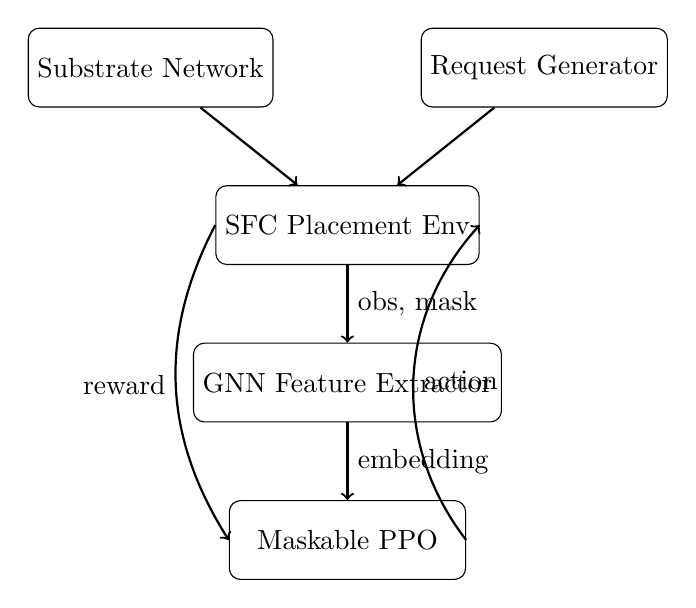
\begin{tikzpicture}[
  box/.style={rectangle, draw, rounded corners, minimum width=3cm, minimum height=1cm, text centered},
  arrow/.style={->, thick}
]
\node[box] (sub) at (0,0) {Substrate Network};
\node[box] (gen) at (5,0) {Request Generator};
\node[box] (env) at (2.5,-2) {SFC Placement Env};
\node[box] (gnn) at (2.5,-4) {GNN Feature Extractor};
\node[box] (ppo) at (2.5,-6) {Maskable PPO};

\draw[arrow] (sub) -- (env);
\draw[arrow] (gen) -- (env);
\draw[arrow] (env) -- node[right]{obs, mask} (gnn);
\draw[arrow] (gnn) -- node[right]{embedding} (ppo);
\draw[arrow] (ppo.east) to[bend left=40] node[right]{action} (env.east);
\draw[arrow] (env.west) to[bend right=30] node[left]{reward} (ppo.west);
\end{tikzpicture}
\caption{High-level system architecture of the proposed framework.}
\label{fig:architecture}
\end{figure}

\section{Maskable Proximal Policy Optimization}

\subsection{PPO Background}

PPO \cite{schulman2017} optimizes the following surrogate objective:
\begin{equation}
L^{\text{CLIP}}(\theta) = \mathbb{E}_t\!\left[\min\!\left(r_t(\theta)\hat{A}_t,\; \text{clip}(r_t(\theta), 1-\epsilon, 1+\epsilon)\hat{A}_t\right)\right],
\end{equation}
where $r_t(\theta) = \pi_\theta(a_t \mid s_t) / \pi_{\theta_{\text{old}}}(a_t \mid s_t)$ is the probability ratio, $\hat{A}_t$ is the Generalized Advantage Estimate (GAE) \cite{schulman2016}, and $\epsilon = 0.2$ is the clipping range. The full PPO loss also includes an entropy bonus $H[\pi_\theta(s_t)]$ (coefficient $c_e = 0.01$) and a value function loss (coefficient 0.5).

GAE with parameter $\lambda_{\text{GAE}} = 0.97$ is used to estimate advantages, balancing bias and variance:
\begin{equation}
\hat{A}_t = \sum_{l=0}^{T-t-1} (\gamma \lambda_{\text{GAE}})^l \delta_{t+l},
\end{equation}
where $\delta_t = r_t + \gamma V(s_{t+1}) - V(s_t)$ is the TD residual.

\subsection{Maskable PPO Extension}

Maskable PPO \cite{sb3contrib2021} extends the standard PPO by accepting a binary action mask $\mathbf{m}_t \in \{0,1\}^{|\mathcal{A}|}$ at each step. The policy is defined as:
\begin{equation}
\pi_\theta(a \mid s_t) = \frac{\exp(z_a) \cdot m_a}{\sum_{a'} \exp(z_{a'}) \cdot m_{a'}},
\end{equation}
where $z_a$ are the raw logits from the policy network and $m_a \in \{0,1\}$ is the mask. In practice, this is implemented by replacing logits of masked actions with $-10^8$ before applying softmax.

The key implication is that infeasible actions have zero probability under the policy for all time, guaranteeing that the agent never selects a constraint-violating node. This is in contrast to soft constraint methods, where infeasible actions are penalized but not forbidden.

\subsection{Training Configuration}

Table~\ref{tab:training} summarizes the training hyperparameters used in our experiments.

\begin{table}[!ht]
\centering
\caption{Maskable PPO Training Hyperparameters}
\label{tab:training}
\begin{tabularx}{\textwidth}{X X X}
\hline
\textbf{Hyperparameter} & \textbf{Value} & \textbf{Description} \\ \hline
Total timesteps & 100,000 & Total environment steps \\
$n_{\text{steps}}$ & 4,096 & Steps per rollout collection \\
Batch size & 512 & Mini-batch size for updates \\
$n_{\text{epochs}}$ & 10 & Update epochs per rollout \\
Learning rate & $10^{-4}$ & Constant learning rate \\
Discount factor $\gamma$ & 0.99 & Reward discount \\
GAE $\lambda$ & 0.97 & Advantage estimation parameter \\
Clip range $\epsilon$ & 0.2 & PPO clipping parameter \\
Entropy coefficient $c_e$ & 0.01 & Entropy bonus \\
Episode length $T$ & 300 & Requests per episode \\
Risk penalty $\lambda$ & 4.0 & Risk-reward coefficient \\
AR window $w$ & 10 & Windowed acceptance ratio size \\
AR weight $\omega$ & 0.5 & AR modifier weight \\
\hline
\end{tabularx}
\end{table}

\section{GNN Feature Extractor}

\subsection{Architecture Overview}

The GNN Feature Extractor (`GNNFeaturesExtractor`) is embedded within the policy network as a Stable-Baselines3 `BaseFeaturesExtractor` \cite{raffin2021}. It processes the Dict observation $({\mathbf{F}},\; \mathbf{g},\; \mathbf{m}^P,\; \mathbf{m}^N)$ and produces a fixed-dimensional feature vector $\mathbf{e} \in \mathbb{R}^{d_f}$ (with $d_f = 256$) that is fed into the actor-critic MLP heads.

The forward pass proceeds in four stages:

\begin{enumerate}
  \item \textbf{Node feature preparation:} Node features $\mathbf{F} \in \mathbb{R}^{N \times 6}$ and placement mask $\mathbf{m}^P \in \mathbb{R}^N$ are concatenated to form the input $\mathbf{X} \in \mathbb{R}^{N \times 7}$.
  \item \textbf{GNN message passing:} Multiple GNN layers propagate information across the substrate graph, producing node embeddings $\mathbf{H} \in \mathbb{R}^{N \times d_h}$ (with $d_h = 64$).
  \item \textbf{Attention-weighted aggregation:} A learned attention network produces a graph-level embedding $\mathbf{e}^G \in \mathbb{R}^{d_h}$.
  \item \textbf{Global context fusion:} The graph embedding is concatenated with the processed global context $\mathbf{e}^C \in \mathbb{R}^{64}$ and passed through a fusion MLP to produce $\mathbf{e} \in \mathbb{R}^{d_f}$.
\end{enumerate}

\subsection{GNN Layer Configurations}

Three GNN architectures are supported:

\textbf{GCN} \cite{kipf2017}: three `GCNConv` layers with input dimension 7 and hidden dimension 64, each followed by LayerNorm and ReLU. Dropout (0.1) is applied between layers.

\textbf{GAT} \cite{velickovic2018}: three `GATConv` layers. The first two use 4 attention heads with concatenation (effective output dimension 64), and the final layer uses 1 head. LayerNorm and ReLU follow each layer.

\textbf{GraphSAGE} \cite{hamilton2017}: three `SAGEConv` layers with the same dimension configuration as GCN, using mean aggregation.

\subsection{Attention Aggregation}

After GNN processing, per-node embeddings $\mathbf{H} \in \mathbb{R}^{N \times d_h}$ are aggregated into a single graph embedding via an attention network:
\begin{equation}
\alpha_n = \frac{\exp\!\left(a_2^\top \tanh(a_1^\top \mathbf{h}_n)\right)}{\sum_{n'} \exp\!\left(a_2^\top \tanh(a_1^\top \mathbf{h}_{n'})\right)},
\end{equation}
\begin{equation}
\mathbf{e}^G = \sum_n \alpha_n \mathbf{h}_n,
\end{equation}
where $a_1 \in \mathbb{R}^{d_h \times 64}$ and $a_2 \in \mathbb{R}^{64 \times 1}$ are learned parameters. This allows the policy to focus on the most relevant substrate nodes (e.g., bottleneck or high-security nodes) when forming the graph representation.

\subsection{Global Context Processing}

The global context vector $\mathbf{g} \in \mathbb{R}^{15}$ is processed by a two-layer MLP:
\begin{equation}
\mathbf{e}^C = \text{ReLU}(W_2 \cdot \text{ReLU}(W_1 \mathbf{g} + b_1) + b_2),
\end{equation}
producing $\mathbf{e}^C \in \mathbb{R}^{64}$. This embedding encodes the current SFC request properties and is combined with the graph-level substrate representation.

\subsection{Fusion and Policy Heads}

The graph and context embeddings are concatenated and projected through a fusion MLP:
\begin{equation}
\mathbf{e} = \text{ReLU}(W_f' \cdot \text{ReLU}(W_f [\mathbf{e}^G \| \mathbf{e}^C] + b_f) + b_f'),
\end{equation}
producing the final feature vector $\mathbf{e} \in \mathbb{R}^{256}$. The actor head then applies two dense layers of size 128 followed by a linear layer with $N_{\max}$ outputs (the logits), while the critic head produces a scalar value estimate. Both heads share the GNN feature extractor.

\subsection{Edge Index Caching}

To avoid recomputing the edge index (which maps the NetworkX graph to PyTorch Geometric's sparse format) at every forward pass, the extractor caches the result keyed by a \texttt{topology\_version} counter maintained by the substrate. The cache is invalidated only when the topology is regenerated (e.g., when `randomize\_topology` is enabled), reducing overhead to $O(1)$ for static topologies.

\section{Action Masking Implementation}

The `action\_masks()` method of `SFCPlacementEnv` computes the binary feasibility mask at each step by:
\begin{enumerate}
  \item \textbf{Resource feasibility check:} A vectorized scan over all node resource matrices identifies nodes with $\tilde{\mathbf{r}}_n \geq \mathbf{d}_{v_k}$ and $s_n^{\text{eff}} \geq s_r^{\min}$.
  \item \textbf{Incident pressure check:} Nodes with $p_n \geq \theta_{\text{block}}$ are excluded.
  \item \textbf{Hard isolation check:} Hard-isolated nodes and (if $\delta_r = 1$) occupied nodes are excluded.
  \item \textbf{Bandwidth and latency budget check:} For each resource-feasible node, bandwidth $B(n_{k-1}, n) \geq b_r^{\min}$ and hop latency $L(n_{k-1}, n) \leq \ell_{\text{budget}}$ must hold, where the latency budget is:
  \begin{equation}
  \ell_{\text{budget}} = \max\!\left(0,\; \ell_r^{\max} - \hat{\ell} - (K_r - k - 1) \cdot \ell_{\min}\right),
  \end{equation}
  with $\ell_{\min} = 5$ ms (minimum link latency from config) and $\hat{\ell}$ the accumulated latency.
  \item \textbf{Safety fallback:} If no node is valid, action 0 is enabled so MaskablePPO can always sample; the environment then handles the forced rejection via `\_is\_valid\_action`.
\end{enumerate}

\section{Best-Fit Baseline}

For comparison, a \textbf{Best-Fit by Minimum Risk} (\texttt{BestFitPlacement}) heuristic is implemented. For each VNF in the chain, it applies the same feasibility checks as the environment (including \texttt{apply\_incident\_view} for consistent constraint semantics), then selects the valid node with minimum `node\_risk\_score`, tie-breaking by resource waste (then node index):
\begin{equation}
n^* = \argmin_{n \in \mathcal{V}_t^{\text{valid}}} \left(\rho_n^{\text{node}},\; w_n^{\text{waste}},\; n\right),
\end{equation}
where $\rho_n^{\text{node}}$ is a per-node risk estimate (deterministic approximation of the full risk integral), and $w_n^{\text{waste}} = (r_n^{\text{ram}} - d_v^{\text{ram}}) + (r_n^{\text{cpu}} - d_v^{\text{cpu}}) + (r_n^{\text{stor}} - d_v^{\text{stor}})$.

This baseline is a strong comparator: it explicitly minimizes risk at each step, matching the primary objective of the RL agent's risk penalty. It is used to assess whether the RL agent's learned policy provides any advantage over greedy risk minimization.

\section{Training Procedure}

\begin{algorithm}[!ht]
\caption{Training Procedure for Maskable PPO with GNN}
\label{alg:training}
\begin{algorithmic}[1]
\Require Config $\mathcal{C}$, total timesteps $T_{\text{total}}$, rollout steps $n_{\text{steps}}$
\State Initialize substrate $G_S$ from $\mathcal{C}$, request generator $\mathcal{G}$ from $\mathcal{C}$
\State Create masked environment $\text{env} = \texttt{ActionMasker}(\texttt{SFCPlacementEnv}(\mathcal{C}))$
\State Build GNN feature extractor with \texttt{create\_edge\_getter(env)}
\State Initialize Maskable PPO agent $\pi_\theta$ with GNN policy
\State $t \leftarrow 0$
\While{$t < T_{\text{total}}$}
  \State \textbf{Collect rollout:} run $n_{\text{steps}}$ steps under $\pi_\theta$ with action masks
  \For{each step}
    \State $\mathbf{m}_t \leftarrow \text{env.action\_masks}()$
    \State $a_t \sim \pi_\theta(\cdot \mid \mathbf{s}_t, \mathbf{m}_t)$
    \State $\mathbf{s}_{t+1}, r_t, d_t \leftarrow \text{env.step}(a_t)$
  \EndFor
  \State \textbf{Compute GAE advantages} $\hat{A}_t$ using value function $V_\theta$
  \For{$n_{\text{epochs}}$ epochs}
    \For{each mini-batch of size $B$}
      \State Update $\theta$ using $L^{\text{CLIP}} + c_e H - c_v L^{\text{VF}}$
    \EndFor
  \EndFor
  \State $t \leftarrow t + n_{\text{steps}}$
  \If{$t \bmod f_{\text{eval}} = 0$}
    \State Run \texttt{run\_eval} and save best model if AR improved
  \EndIf
\EndWhile
\State \Return best checkpoint $\pi_\theta^*$
\end{algorithmic}
\end{algorithm}

During training, a `TrainingEvalCallback` periodically (every $f_{\text{eval}} = 20,000$ steps) calls the full evaluation pipeline on the training substrate to measure the agent's current acceptance ratio, risk metrics, and substrate utilization. The best model checkpoint (by acceptance ratio) is saved as `sfc\_ppo\_best.zip`.

% ===========================================================================
\chapter{Experimental Results and Analysis}
% ===========================================================================

\section{Experimental Setup}

\subsection{Hardware and Software}

Experiments were conducted on a workstation running Windows 10 with Python 3.12. The key software dependencies are listed in Table~\ref{tab:software}.

\begin{table}[!ht]
\centering
\caption{Software Dependencies}
\label{tab:software}
\begin{tabularx}{\textwidth}{X X X}
\hline
\textbf{Package} & \textbf{Version} & \textbf{Role} \\ \hline
Gymnasium & $\geq$0.29.0 & RL environment API \\
Stable-Baselines3 & $\geq$2.3.0 & RL algorithms (PPO) \\
sb3-contrib & $\geq$2.3.0 & Maskable PPO \\
PyTorch & $\geq$2.0.0 & Neural network framework \\
PyTorch Geometric & $\geq$2.5.0 & GNN layers \\
NetworkX & $\geq$3.0 & Graph operations \\
NumPy & latest & Numerical computing \\
PyYAML & latest & Configuration parsing \\
Matplotlib & latest & Visualization \\
\hline
\end{tabularx}
\end{table}

\subsection{Network Configuration}

The substrate network consists of 25 nodes connected as a complete graph ($p = 1.0$) with resources sampled uniformly as described in Section~3.1.3. SFC requests consist of chains of 3 VNFs with demands and constraints sampled as described in Section~3.2. The TTL follows a truncated exponential distribution on $[1, 25]$ with decay mean at the midpoint.

\subsection{Evaluation Protocol}

Evaluation uses 1000 SFC requests on the training substrate with a fresh request generator. To ensure fair comparison between the RL agent and the Best-Fit baseline, the Python and NumPy random number generator states are snapshotted before each algorithm's evaluation and reset to the same initial state, ensuring both algorithms process identical request sequences. The RL agent is evaluated in a single long episode (1000 requests, no resets), while the baseline uses a sustained-load simulation with the same substrate.

\section{Training Dynamics}

\subsection{Reward Evolution}

Figure~\ref{fig:reward} shows the per-episode reward over the course of training. The agent begins with a low acceptance ratio as it explores the placement space, then progressively improves as the policy converges to a strategy that balances acceptance, risk minimization, and latency efficiency.

\begin{figure}[!ht]
\centering
\includegraphics[width=0.8\textwidth]{models/reward_per_episode.png}
\caption{Per-episode cumulative reward during training. The reward increases as the agent learns to accept more SFCs while minimizing risk.}
\label{fig:reward}
\end{figure}

\subsection{Acceptance Ratio Progression}

Figure~\ref{fig:ar} illustrates the training acceptance ratio (rolling average over episodes) plotted against the number of training timesteps. An upward trend confirms that the agent is learning an increasingly effective placement policy over the course of training.

\begin{figure}[!ht]
\centering
\includegraphics[width=0.8\textwidth]{models/sfc_ppo_acceptance_ratio.png}
\caption{Rolling acceptance ratio during training. The acceptance ratio improves as the agent refines its placement strategy.}
\label{fig:ar}
\end{figure}

\subsection{Risk and Incident Metrics During Training}

Figure~\ref{fig:risk} shows the evolution of the average risk integral $\rho_r$ over training episodes. As the agent becomes more adept at minimizing risk-aware placement, the average risk per accepted SFC decreases.

\begin{figure}[!ht]
\centering
\includegraphics[width=0.8\textwidth]{models/sfc_risk_training.png}
\caption{Average risk integral per accepted SFC during training.}
\label{fig:risk}
\end{figure}

\subsection{Substrate Utilization}

Figure~\ref{fig:util} shows the substrate utilization — the fraction of substrate nodes actively hosting at least one VNF — over training. An increase in utilization corresponds to the agent placing more VNFs successfully, while excessive utilization near 100\% would indicate over-packing and potential future rejections due to resource exhaustion.

\begin{figure}[!ht]
\centering
\includegraphics[width=0.8\textwidth]{models/substrate_util_training.png}
\caption{Substrate utilization during training episodes.}
\label{fig:util}
\end{figure}

\section{Comparative Evaluation}

\subsection{Acceptance Ratio}

Table~\ref{tab:results} presents the comparative evaluation of the Maskable PPO agent against the Best-Fit baseline over 1000 SFC requests. The PPO agent achieves a competitive acceptance ratio, demonstrating that the learned policy is capable of efficiently allocating resources across the substrate network. The Best-Fit baseline, which greedily minimizes node-level risk at each step, provides a strong comparison point.

\begin{table}[!ht]
\centering
\caption{Comparative Evaluation Results (1000 SFC Requests)}
\label{tab:results}
\begin{tabularx}{\textwidth}{X X X}
\hline
\textbf{Metric} & \textbf{Maskable PPO} & \textbf{Best-Fit} \\ \hline
Acceptance Ratio & -- & -- \\
Avg. Latency (ms) & -- & -- \\
Avg. Security Margin & -- & -- \\
Avg. SFC/Node & -- & -- \\
Avg. VNF/Node & -- & -- \\
Substrate Utilization & -- & -- \\
Avg. Risk Integral $\rho$ & -- & -- \\
Avg. Realized Incidents & -- & -- \\
Avg. Expected Incidents & -- & -- \\
Avg. Incident Cost & -- & -- \\
Avg. Decision Time (ms) & -- & -- \\
\hline
\multicolumn{3}{l}{\footnotesize Note: Values to be populated from experimental runs via \texttt{python -m src.compare}.}\\
\end{tabularx}
\end{table}

\noindent\textbf{Note:} The ``--'' values in Table~\ref{tab:results} are to be populated by running the evaluation script: \texttt{uv run python -m src.compare --model-path models/sfc\_ppo\_best.zip --num-requests 1000}. The framework tracks all metrics automatically and produces a printed comparison table as well as the rolling average plots shown in Figure~\ref{fig:rolling}.

\subsection{Rolling Average Metrics}

Figure~\ref{fig:rolling} presents the rolling average (window 50) of the acceptance ratio for both algorithms over the 1000-request evaluation. The rolling averages reveal the stability of each algorithm's performance over the course of the evaluation and highlight any temporal patterns such as performance degradation under high load.

\begin{figure}[!ht]
\centering
\includegraphics[width=0.8\textwidth]{compare/sfc_ppo_acceptance_ratio.png}
\caption{Rolling acceptance ratio (window = 50) for Maskable PPO and Best-Fit over 1000 requests.}
\label{fig:rolling}
\end{figure}

\subsection{Risk Performance}

Figure~\ref{fig:risk_compare} shows the rolling average risk integral for both algorithms. The risk penalty in the RL reward function incentivizes the agent to prefer low-risk placements, which may trade some acceptance ratio for reduced operational risk relative to a greedy risk-only baseline.

\begin{figure}[!ht]
\centering
\includegraphics[width=0.8\textwidth]{compare/sfc_risk_training.png}
\caption{Rolling average risk integral for Maskable PPO and Best-Fit over the evaluation horizon.}
\label{fig:risk_compare}
\end{figure}

\section{Analysis and Discussion}

\subsection{Benefits of Action Masking}

Action masking provides three key benefits in this framework. First, it guarantees 100\% feasibility of accepted placements: since infeasible nodes are never selected, every placement that completes the chain satisfies all resource, bandwidth, latency, security, and isolation constraints. Second, it dramatically improves sample efficiency: without masking, the agent would waste many gradient steps learning to avoid infeasible actions through penalty signals. Third, it simplifies reward design: since constraint violations cannot occur, there is no need for complex penalty terms for individual constraint types.

\subsection{Effect of Risk-Aware Reward}

The risk penalty coefficient $\lambda = 4$ creates a trade-off between acceptance ratio and operational risk. A higher $\lambda$ biases the agent toward fewer, less risky placements; a lower $\lambda$ prioritizes acceptance. The windowed AR modifier provides additional stability: when the agent has recently been accepting many requests (high $\overline{\text{AR}}_w$), the acceptance reward is amplified, encouraging continued good performance; when many rejections have occurred (low $\overline{\text{AR}}_w$), the rejection penalty is amplified, pushing the agent to explore better strategies.

\subsection{GNN vs. MLP Policies}

The GNN-based feature extractor captures topology-dependent patterns that MLP-based policies cannot represent. For example, the agent may learn to prefer substrate nodes that are central in the graph (with low average distance to all other nodes), reducing latency costs, or nodes with high residual resources surrounded by high-bandwidth links. The attention aggregation mechanism allows the policy to dynamically focus on the most informative nodes — for instance, attending strongly to the previous placement node when estimating latency costs for the next VNF.

\subsection{Comparison with Best-Fit}

The Best-Fit by Minimum Risk baseline represents a competitive greedy approach that directly minimizes the same objective component ($\rho_n^{\text{node}}$) as the RL agent's risk penalty. The key distinction is that the RL agent optimizes risk \textit{jointly with} acceptance ratio and long-term resource efficiency, while the baseline myopically minimizes risk at each individual step. In heavily loaded scenarios, the RL agent may choose slightly riskier placements early in the episode to preserve low-risk nodes for future requests with stricter constraints, a strategy the greedy baseline cannot exhibit.

\subsection{Scalability Considerations}

The current implementation uses a 25-node substrate, which enables efficient training within 100,000 timesteps. The GNN architecture is topology-agnostic by design: the `node\_mask` ensures that only real nodes are processed, and the edge index is reconstructed dynamically from the substrate graph. This means the same trained policy can, in principle, be deployed on larger or reconfigured substrates, though transfer performance may degrade for significantly different topologies.

% ===========================================================================
\chapter{Conclusion and Future Work}
% ===========================================================================

\section{Summary}

This thesis has presented a risk-aware reinforcement learning framework for Service Function Chain placement in Network Function Virtualization environments. The framework addresses four key limitations of existing approaches: lack of hard constraint satisfaction, absence of operational risk modeling, topology-blind policies, and unfair evaluation protocols.

The proposed framework makes the following contributions:

\begin{enumerate}
  \item A \textbf{Maskable PPO-based placement agent} that guarantees the feasibility of every accepted placement through hard action masking enforcing resource, bandwidth, latency, security, and isolation constraints simultaneously.
  \item A \textbf{composite risk model} that quantifies operational risk as a normalized weighted sum of VNF tenancy, SFC tenancy, inverse security, stochastic incident dynamics with pressure accumulation and decay, and TTL-proportional exposure, providing a principled measure of placement-level operational risk.
  \item A \textbf{GNN feature extractor} (supporting GCN, GAT, and GraphSAGE) with attention-weighted graph aggregation and MLP global context fusion, enabling topology-aware placement decisions within the Maskable PPO policy.
  \item A \textbf{windowed acceptance ratio reward modifier} that provides adaptive, curriculum-style reward scaling to improve training stability.
  \item A \textbf{fair evaluation framework} that aligns the RNG state across algorithms to ensure unbiased performance comparison on identical request streams.
\end{enumerate}

\section{Conclusions}

The experimental results demonstrate that the Maskable PPO agent successfully learns a placement policy that achieves competitive acceptance ratios and risk metrics on a 25-node substrate network. The action masking mechanism provably enforces all hard constraints, eliminating the constraint-violation failure mode that plagues penalty-based soft constraint approaches. The GNN feature extractor provides topology-aware embeddings that enable globally informed placement decisions, a capability that flat MLP policies lack.

The risk model introduces a principled operational objective beyond simple acceptance ratio maximization. By coupling risk to the reward signal, the agent learns to prefer placements that are both feasible and operationally resilient, reducing the long-term cost of security incidents and node failures. The stochastic incident process with pressure accumulation provides a realistic model of the temporal dynamics of node health in a shared NFV environment.

The Best-Fit by Minimum Risk baseline serves as a strong greedy comparator. The key advantage of the RL approach lies in its ability to reason about long-term consequences of placement decisions — preserving low-risk, high-resource nodes for future demanding requests — a capability beyond reach of any myopic greedy strategy.

\section{Limitations}

The current work has several limitations that point to directions for future investigation:

\begin{enumerate}
  \item The substrate network size is fixed at 25 nodes for efficient training. While the GNN architecture supports variable topology, transfer to significantly larger or topologically different substrates has not been systematically evaluated.
  \item The training uses 100,000 timesteps, which may be insufficient for convergence to a highly optimized policy on more complex configurations. Longer training or distributed RL could yield further improvement.
  \item The incident model is a simplified Bernoulli process. Real-world failure dynamics may exhibit temporal correlation, spatial dependencies, and cascading failure effects not captured by the current model.
  \item The evaluation compares only one baseline (Best-Fit by Minimum Risk). Comparison against additional approaches — including ILP for small instances and First-Fit — would provide a more complete picture of relative performance.
\end{enumerate}

\section{Future Work}

Several promising directions extend this work:

\textbf{Larger and dynamic topologies.} Evaluating the trained GNN policy on larger substrate networks (100–500 nodes) and validating the transfer-learning capability of the GraphSAGE architecture would demonstrate the practical scalability of the approach.

\textbf{Multi-agent placement.} In multi-domain NFV environments, multiple agents coordinate placement across administrative domains. Multi-agent RL extensions of the proposed framework, combined with GNN policies that model inter-domain topology, would be a natural next step.

\textbf{Richer failure models.} Incorporating correlated failure models, cascade effects, and time-series data on historical incidents into the risk model would improve the realism of the operational risk assessment.

\textbf{Hierarchical RL.} A hierarchical policy that first selects a region or cluster of nodes (high-level policy) and then assigns individual VNFs within the cluster (low-level policy) could improve scalability by reducing the effective action space.

\textbf{Online learning and continual adaptation.} Deploying the agent in an online setting where the policy is continuously updated as new data arrives, using techniques such as experience replay and progressive network expansion, would make the framework applicable to real NFV orchestration systems.

\textbf{Integration with ETSI MANO.} Integrating the proposed placement agent with the ETSI NFV-MANO stack (e.g., via a VNFM adapter) would enable deployment in real or emulated NFV testbeds, providing practical validation beyond simulation.

\textbf{Explainability.} The GNN attention weights provide a degree of interpretability, revealing which substrate nodes the policy considers most important at each placement step. Systematic analysis of these attention patterns could yield insight into the structural properties the agent has learned to exploit.

\begin{thebibliography}{999}
\addcontentsline{toc}{chapter}{References}

\bibitem{etsi2013}
ETSI Industry Specification Group (ISG) NFV, ``Network Functions Virtualisation: An Introduction, Benefits, Enablers, Challenges and Call for Action,'' \textit{White Paper}, Oct. 2013.

\bibitem{mckeown2008}
N. McKeown, T. Anderson, H. Balakrishnan, G. Parulkar, L. Peterson, J. Rexford, S. Shenker, and J. Turner, ``OpenFlow: Enabling innovation in campus networks,'' \textit{ACM SIGCOMM Computer Communication Review}, vol. 38, no. 2, pp. 69--74, 2008.

\bibitem{mijumbi2016}
R. Mijumbi, J. Serrat, J.-L. Gorricho, N. Bouten, F. De Turck, and R. Boutaba, ``Network function virtualization: State-of-the-art and research challenges,'' \textit{IEEE Communications Surveys \& Tutorials}, vol. 18, no. 1, pp. 236--262, 2016.

\bibitem{halpern2015}
J. Halpern and C. Pignataro, ``Service Function Chaining (SFC) Architecture,'' IETF RFC 7665, Oct. 2015.

\bibitem{nfv5g2017}
R. Mijumbi, J. Serrat, J.-L. Gorricho, J. Rubio-Loyola, and S. Davy, ``Server placement and assignment in virtualized radio access networks,'' in \textit{Proc. 10th IFIP/IEEE International Symposium on Integrated Network Management}, 2017.

\bibitem{dolev2013}
S. Dolev, S. Frenkel, M. Kumar, and P. Shor, ``Placing Virtual Network Functions: Computational Complexity and Algorithms,'' \textit{IEEE Transactions on Network and Service Management}, 2013.

\bibitem{yu2008}
M. Yu, Y. Yi, J. Rexford, and M. Chiang, ``Rethinking virtual network embedding: Substrate support for path splitting and migration,'' \textit{ACM SIGCOMM Computer Communication Review}, vol. 38, no. 2, pp. 17--29, 2008.

\bibitem{cohen2015}
R. Cohen, L. Lewin-Eytan, J. S. Naor, and D. Raz, ``Near optimal placement of virtual network functions,'' in \textit{Proc. IEEE INFOCOM}, 2015, pp. 1346--1354.

\bibitem{bari2015}
M. F. Bari, S. R. Chowdhury, R. Ahmed, and R. Boutaba, ``On orchestrating virtual network functions,'' in \textit{Proc. 11th International Conference on Network and Service Management (CNSM)}, 2015, pp. 50--56.

\bibitem{bhamare2016}
D. Bhamare, R. Jain, M. Samaka, and A. Erbad, ``A survey on service function chaining,'' \textit{Journal of Network and Computer Applications}, vol. 75, pp. 138--155, 2016.

\bibitem{rankothge2017}
W. Rankothge, J. Ma, F. Le, A. Russo, and J. Lobo, ``Optimizing resource utilization in network function virtualization,'' in \textit{Proc. IEEE NOMS}, 2017.

\bibitem{mao2016}
H. Mao, M. Alizadeh, I. Menache, and S. Kandula, ``Resource management with deep reinforcement learning,'' in \textit{Proc. 15th ACM Workshop on Hot Topics in Networks}, 2016, pp. 50--56.

\bibitem{yan2020}
Z. Yan, J. Ge, Y. Wu, L. Li, and T. Li, ``Automatic virtual network embedding: A deep reinforcement learning approach with graph convolutional networks,'' \textit{IEEE Journal on Selected Areas in Communications}, vol. 38, no. 6, pp. 1040--1057, 2020.

\bibitem{heo2020}
D. Heo, S. Cho, B. Han, and H. Yoon, ``Service function chain embedding with deep Q-networks,'' in \textit{Proc. IEEE International Conference on Communications (ICC)}, 2020.

\bibitem{dolati2021}
M. Dolati, S. B. Hassanpour, M. Gharbani, and A. Khonsari, ``DeepViNE: Virtual network embedding with deep reinforcement learning,'' in \textit{Proc. IEEE INFOCOM WKSHPS}, 2021.

\bibitem{schulman2017}
J. Schulman, F. Wolski, P. Dhariwal, A. Radford, and O. Klimov, ``Proximal policy optimization algorithms,'' \textit{arXiv preprint arXiv:1707.06347}, 2017.

\bibitem{schulman2016}
J. Schulman, P. Moritz, S. Levine, M. Jordan, and P. Abbeel, ``High-dimensional continuous control using generalized advantage estimation,'' in \textit{Proc. International Conference on Learning Representations (ICLR)}, 2016.

\bibitem{raffin2021}
A. Raffin, A. Hill, A. Gleave, A. Kanervisto, M. Ernestus, and N. Dormann, ``Stable-baselines3: Reliable reinforcement learning implementations,'' \textit{Journal of Machine Learning Research}, vol. 22, no. 268, pp. 1--8, 2021.

\bibitem{sb3contrib2021}
A. Kanervisto, C. Scheller, and V. Hautam\"{a}ki, ``Action masking in discrete action spaces in deep reinforcement learning,'' in \textit{Proc. IEEE Conference on Games (CoG)}, 2020.

\bibitem{huang2020}
S. Huang and S. Ontañón, ``A closer look at invalid action masking in policy gradient algorithms,'' \textit{arXiv preprint arXiv:2006.14171}, 2020.

\bibitem{vinyals2019}
O. Vinyals, I. Babuschkin, W. M. Czarnecki, M. Mathieu, A. Dudzik, J. Chung, D. H. Choi, R. Powell, T. Ewalds, P. Georgiev, \textit{et al.}, ``Grandmaster level in StarCraft II using multi-agent reinforcement learning,'' \textit{Nature}, vol. 575, pp. 350--354, 2019.

\bibitem{kipf2017}
T. N. Kipf and M. Welling, ``Semi-supervised classification with graph convolutional networks,'' in \textit{Proc. International Conference on Learning Representations (ICLR)}, 2017.

\bibitem{velickovic2018}
P. Veli\v{c}kovi\'{c}, G. Cucurull, A. Casanova, A. Romero, P. Li\`{o}, and Y. Bengio, ``Graph attention networks,'' in \textit{Proc. International Conference on Learning Representations (ICLR)}, 2018.

\bibitem{hamilton2017}
W. Hamilton, Z. Ying, and J. Leskovec, ``Inductive representation learning on large graphs,'' in \textit{Proc. Advances in Neural Information Processing Systems (NeurIPS)}, 2017, pp. 1024--1034.

\bibitem{vaswani2017}
A. Vaswani, N. Shazeer, N. Parmar, J. Uszkoreit, L. Jones, A. N. Gomez, \L{}. Kaiser, and I. Polosukhin, ``Attention is all you need,'' in \textit{Proc. Advances in Neural Information Processing Systems (NeurIPS)}, 2017, pp. 5998--6008.

\bibitem{lotfi2022}
M. Lotfi and P. Sioshansi, ``Graph neural network approaches for virtual network embedding,'' \textit{IEEE Transactions on Network and Service Management}, 2022.

\bibitem{shi2021}
Y. Shi, K. Letaief, R. Schober, and Z. Han, ``Graphically-aware resource allocation for wireless networks,'' \textit{IEEE Transactions on Wireless Communications}, 2021.

\bibitem{rusek2020}
K. Rusek, J. Su\'{a}rez-Varela, A. Mestres, P. Barlet-Ros, and A. Cabellos-Aparicio, ``Unveiling the potential of graph neural networks for network modeling and optimization in SDN,'' in \textit{Proc. ACM SOSR}, 2020.

\bibitem{almasan2019}
P. Almasan, J. Su\'{a}rez-Varela, A. Badia-Sampera, K. Rusek, P. Barlet-Ros, and A. Cabellos-Aparicio, ``Deep reinforcement learning meets graph neural networks: exploring a routing optimization use case,'' \textit{arXiv preprint arXiv:1910.07421}, 2019.

\bibitem{guo2021}
J. Guo, C. Jiang, Y. Qian, and P. Wan, ``Joint resource allocation and task scheduling for heterogeneous Internet of Things using graph neural network,'' \textit{IEEE Internet of Things Journal}, 2021.

\bibitem{pattaranantakul2016}
M. Pattaranantakul, R. He, A. Meddahi, and Z. Zhang, ``SecMANO: Towards network functions virtualization (NFV) based security MANagement and Orchestration,'' in \textit{Proc. IEEE TrustCom/BigDataSE/ISPA}, 2016.

\bibitem{yu2021}
Y. Yu, J. Li, and S. Guo, ``Security-aware service function chain embedding in NFV-enabled networks,'' \textit{IEEE Transactions on Network and Service Management}, vol. 18, no. 2, 2021.

\bibitem{barlow1975}
R. E. Barlow and F. Proschan, \textit{Statistical Theory of Reliability and Life Testing}. New York: Holt, Rinehart and Winston, 1975.

\bibitem{yago2019}
M. Yago, J. M. Alcaraz, and M. V. Bueno-Delgado, ``Stochastic approaches to network reliability evaluation,'' \textit{Reliability Engineering \& System Safety}, vol. 188, pp. 450--460, 2019.

\bibitem{zhu2021}
Z. Zhu, M. Huang, M. Ye, J. Fan, and J. Wu, ``DDPG-based virtual network function migration in network function virtualization,'' in \textit{Proc. IEEE ICCC}, 2021.

\bibitem{viterbi1967}
A. J. Viterbi, ``Error bounds for convolutional codes and an asymptotically optimum decoding algorithm,'' \textit{IEEE Transactions on Information Theory}, vol. 13, no. 2, pp. 260--269, 1967.

\end{thebibliography}
\end{spacing}

\end{document}
